\chapter{Comparison}
\label{ch:compare}
In the previous chapter (cf. Chapter \ref{ch:intro}), we learned how each analysis operates, so now we can begin comparing their approaches.\codyze{} and \cognicryptsast{} use rules that are written in different DSLs, \MARK, and \crysl, respectively.Both tools employ graph structures to represent source code and facilitate the analysis of the code; however, \cognicryptsast{} generates call graphs (CG), whereas \codyze{} generates code property graphs (CPG). \codyze{} creates a CPG from the source code, then analyzes this graph based on the written rules, however, as stated in Section \ref{sec:cc}, \cognicryptsast{} creates a Soot IR from the source code and performs the analysis on the IR, not the source code itself. Therefore, it is important that we take an in-depth examination of the approaches of these tools in order to discover more similarities and differences, as well as the advantages and disadvantages associated with them.

Throughout this chapter, we compare the tools theoretically, then we compare them in practice, and finally, we compare their respective DSLs thoroughly.

\section{Theoretical Comparison of \cognicryptsast{} and \codyze{}}
\label{sec:theotools}
To summarize the previous chapter, \codyze{} \cite{cod} and \cognicryptsast{} \cite{stefanphd} are static analyzers for security testing that analyze the program to find cryptographic misuses. \codyze{} and \cognicryptsast{} consume \MARK{} \cite{cod} and \crysl{} \cite{skm19} rules respectively to perform the analysis. \MARK{} and \crysl{} are both DSLs for specifying the correct usages of cryptographic APIs. We can divide the theoretical comparison of \codyze{} and \cognicryptsast{} into two parts, graph generation and how each tool analyzes the constructed graphs against the rules. Based on the information we provided on each tool on Chapter \ref{ch:intro}, we will compare them closely in analysis and graphs.

\subsection{Comparison of the graphs}
As we discussed in the previous chapter (cf. Chapter \ref{ch:intro}), both tools convert the source code into an intermediate representation in order to facilitate and speed up the analysis process. \codyze{} converts the source code into a graph representation (CPG), and \cognicryptsast{} transforms the source code into a Soot IR (Jimple), and then builds a call graph of the program or combines individual CFGs and the program’s call graph into an ICFG.

The CPG is explicitly designed to identify vulnerabilities in large amounts of source code efficiently and effectively \cite{cpg}. CPG can be generated of an erroneous code. Therefore, \codyze{} can analyze incomplete source codes and tolerate minor syntax errors \cite{cod}. The CPG can either be used manually with a query language (e.g., NQL, SQL, or Gremlin) to identify the relevant patterns or automatically when integrated into CI/CD or IDEs \cite{cod}. CPGs are independent of programming languages. When a program with a specific programming language is translated into a CPG, any query written for any other programming language can also apply to this CPG. Consequently, \codyze{} is capable of analyzing C and C++ programs as well as Java programs.
The Code Property Graph (CPG) combines many representations of source code into one queryable graph database. This enables the CPG to understand the full flow of information across an application (AST) and represents the order in which statements are executed (CFG), and detects flaw injections or leaks of sensitive information (PDG). As a result, \codyze{} is a flow-sensitive data-flow analysis. CPG does not address inter-procedural analysis; however, it can be enhanced with call edges to provide inter-procedural analysis as shown in the study by Backes \etal \cite{cpgphp}.

% However, the order of operations cannot be analyzed with only the query language, therefore codyze developers implemented a typestate analysis for that matter. The valid typestates are determined by regular expression in the MARK "order" construct (see Listing \ref{lst:keygenmarkruletrans} Line \ref{line:ordermark}).


\cognicryptsast{} first parses the programs into an IR (Jimple) using Soot \cite{soot} and then constructs a call graph for it. IRs generally cover a limited number of constructs to analyze a program while still expressing all language elements. These limits simplify analysis by reducing the number
of cases that analysis must cover. This leads to a simpler call graph. Call graphs show an abstraction of all method calls in a program that could be used for further analysis. In addition to call graphs, \cognicryptsast{} constructs CFGs of individual statements and sometimes creates an ICFG to represent the whole program. A similar approach applies to analyzing Android programs intra-procedurally. Moreover, the FlowDroid \cite{flowdroid} extension allows the creation of Android-specific call graphs that can be used to construct the ICFG and perform inter-procedural analysis.
% valid typestates are same as mark determined by regular expression in the ORDER section of the crysl rules (see Listing \ref{lst:orgkeygencrysl} line \ref{line:ordercrysl})

% In this thesis we will chose the CHA call graphs the default algorithm for evaluating cognicryptsast 
% (cf. \ref{ch:eval}) cause although it is not precise but is efficient and is context sensitive.
Currently, Soot only accepts Java code as an input to make IR, and therefore, \cognicryptsast{} cannot analyze other languages since it lacks the required IR. According to the readme file of the Soot Github repository \cite{sootgit}, Soot can process Java code up to Java 9. However, the Soot documentation page has not been updated and indicates that it only supports Java code up to Java 7 \cite{soot}. \cognicryptsast{} have not been modified yet to use the most recent version of Soot and can only work with Java source code up to Java 8, and cannot analyze programs with Java versions higher than Java 8.


The graph construction is the most time-consuming part of the analysis in \cognicryptsast. According to \cite{skm19}, the majority of the total analysis time (83\%) is spent on call graph construction in analyzing 8,422 apps by \cognicryptsast{}. There are no publications or resources available to illustrate the time required to generate a CPG in \codyze{}, except for a presentation \cite{presentationcodyze} which included statistics of a \codyze{} analysis of 338 KB C++ source codes (12K lines of code and 486 methods). Based on their calculations, the CPG conversion time was 2.7 seconds or approximately 6 percent of the total analysis time. The results are unreliable to predict how much time will be required to construct a CPG on average. For this purpose, we would need to generate CPG for a significant number of programs to provide an accurate estimate. Upon further research on the CPG, we discovered that Backes \etal{} \cite{cpgphp} generated CPGs with the call edges of 1,854 projects in their study. The results show that the AST generation of all projects took 40 minutes and 30 seconds, and the CFG, PDG, and call edge generations took 5 hours 10 minutes 33 seconds. However, this does not provide a reasonable estimate of how long it takes to generate a CPG since they did not create a pure CPG. We could further calculate the average time it takes to create a CPG using \codyze{} by analyzing several benchmarks and calculating the time required to create the CPG. This, however, was beyond the scope of our thesis as it involved a few modifications to \codyze's source code, which would require some time and, therefore, exceed our time limits. We will discuss it further in the further work chapter (cf. Chapter \ref{ch:fwork}).

CPG is more complex and sophisticated than CG. \codyze{} extracts most of the analysis information directly from the CPG with the help of a query language to verify that it complies with the \MARK{} rules, whereas \cognicryptsast{} performs three different analyses on the call graph to determine whether it complies with the \crysl{} rules (cf. chapter \ref{ch:intro}). Using only the query language is not sufficient for analyzing the order of operations in \codyze. Therefore, \codyze{} developers have implemented a typestate analysis for this purpose. We will discuss this in the next section (Section \ref{sec:comanalysis}).

In order to determine which approach is more precise and effective, we will compare the results of the analysis performed by each tool with the same rules (same API specifications but with different DSLs) and the same source code in the Evaluation chapter (cf. Chapter \ref{ch:eval}). 

\subsection{Comparison of the analysis of the graphs}
\label{sec:comanalysis}
In the previous section, we discussed the graphs and the intermediate representations of the source code that each tool generates. In this section, we will examine the analyses that \codyze{} and \cognicryptsast{} perform on the IRs in order to identify cryptographic misuses in the program. As mentioned in the Chapter \ref{ch:intro}, \codyze{} and \cognicryptsast{} examine the code against the written \MARK{} and \crysl{} rules, respectively. Both tools have parsers that convert the rules into models that the respective analysis can use.

According to Kreuger \cite{stefanphd}, they have developed a parser for translating \crysl{} rules into the \crysl{} object model. \cognicryptsast{} transforms the rules in the \crysl{} object model into a static data-flow analysis that is both flow- and context-sensitive. \cognicryptsast{} contains a typestate analysis to validate the order in which the operations are called, a Boomerang instance to check the parameters against the \crysl{} rules, and a taint analysis for flaw injections and information leakage in Android applications. The analysis automatically examines Java or Android applications that have been converted into Jimple to determine whether they conform to the encoded \crysl{} rules. The error message that \cognicryptsast{} generates in the event of a misuse depends on the type of misuse and the factors that led to the misuse. There are several types of misuses that we named in Section \ref{sec:cc}. 

\codyze{} converts the \MARK{} rules into a \MARK{} model that the analysis can use. \codyze{} utilizes CPG and query language to analyze a program's data flow and detect information leaks. In \codyze, the order of operations cannot be analyzed with only the query language; as a result, \codyze{} developers implemented a typestate analysis in that regard. \codyze{} error messages are derived from a JSON file created by \codyze{} maintainers (see Section \ref{sec:codyze}), with the exception of order and forbidden call violations. Error messages related to those violations are generated automatically at \codyze's runtime.


Both tools utilize typestate analysis to provide flow sensitivity to ensure that the order of operations in the source code complies with the \MARK{} or \crysl{} rules. Nevertheless, \cognicryptsast{} employs IDE\textsuperscript{al} \cite{IDEal}, a framework for inter-procedural data-flow analysis, in order to perform a typestate analysis. The analysis defines a finite-state machine from the ORDER section of the \crysl{} rule to verify an object's trace in the program. It also defines the allocation sites from which to begin the analysis. An allocation site is a point at which an object is created in an object-oriented program. IDE\textsuperscript{al} performs a flow-, field-, and context-sensitive typestate analysis from those allocation sites. Because C is not an object-oriented language, and C++ is not an entirely object-oriented language, this typestate analysis cannot be used to analyze C programs or all C++ programs.

\codyze, on the other hand, uses a Weighted Pushdown System (WPDS) \cite{pushdown} for typestate analysis. The WPDS presents an abstraction of the data flows within a program. Currently, there is one WPDS per function in \codyze; therefore, it is not inter-procedural. Nonetheless, when evaluating the performance of \codyze, we realized that it is partially inter-procedural. We will discuss it in Chapter \ref {ch:eval}. The typestates are specified by a regular expression in the \MARK{} \code{order} construct. The analysis converts the regular expression into a Non-deterministic Finite Automaton (NFA). The finite automata are called NFA when there exist many paths for specific input from the current state to the next state. Typestate NFA transitions are then represented as weights for a WPDS. This typestate can be used for non-object-oriented programs such as C.

In both tools, valid typestates are determined by regular expressions in the rules. In \crysl, regular expressions are defined in the ORDER section (see Listing \ref{lst:orgkeygencrysl} Line \ref{line:ordercrysl}) and in \MARK, the order construct (see Listing \ref{lst:keygenmarkruletrans} Line \ref{line:ordermark}).

Although we have an understanding of the differences in the implementation of analyzers of both tools, we will only be able to determine the effectiveness of each approach in an evaluation. We, therefore, will perform an evaluation in Chapter \ref{ch:eval}.



\section{Comparison of \cognicryptsast{} and \codyze{} in practice}
\label{sec:practical}
The next step will be to compare and discuss \codyze{} and \cognicryptsast{} in order to identify how they work in practice. This will include which editors and IDEs they support, what error messages they generate, and how they function in practice. As both tools are capable of analyzing Java programs, we have compared the tools for analyzing Java programs; \codyze's analysis of C++ and C programs is left to future research.

\subsubsection*{Setup}
For this comparison, we used two virtual machines that had the same configuration, which means that they had the same hardware specifications (Intel(R) Xeon(R) CPU E5-2695, 2.30GHz machine with 2 virtual processors, 8 GB RAM, and 50 GB hard disc capacity) and the same operating system (Windows 10 Education). On the first machine we installed Java 8 (JDK version 1.8.0\_301) and on the second Java 11 (JDK version 11.0.11) since \codyze{} requires Java 11 or above while \cognicryptsast{} requires Java 8. The Eclipse 2020-06 was installed on both machines since this is the latest version of Eclipse that supports the two Java versions. 
The versions of \codyze{} and \cognicryptsast{} that we used are not the published versions. We downloaded the source code of \cognicryptsast{} and \codyze{} up to the date of 31st of October 2021 and built them on the first and second virtual machines, respectively. We have downloaded the following source codes.
\cognicrypt{} plugin source code on the develop branch to the commit ef64a0f\footnote{\url{https://github.com/eclipse-cognicrypt/CogniCrypt/commit/ef64a0f2aa7bd54fdc70ae518691cfadf7f47f53}} to use the \cognicryptsast{} as part of \cognicrypt{} Eclipse plugin. In addition, the \cognicryptsast{} standalone command-line tool from the develop branch to this commit 35d0916 \footnote{\url{https://github.com/CROSSINGTUD/CryptoAnalysis/commit/35d09163f97b6919a4359fcaa0e846af95c1fed1}}. Lastly, the source code of \codyze{} main branch to the commit 0468af1\footnote{\url{https://github.com/Fraunhofer-AISEC/codyze/commit/0468af19b90b16353402938db4e326b6dc63c4f7}}.

We will later use the same machines to compare the DSLs in the DSL comparison section (Section \ref{sec:dsl}) and evaluate \codyze{} and \cognicryptsast{} performances in the Evaluation chapter (cf. Chapter \ref{ch:eval}).

\subsection*{Discussion}
Currently, \codyze{} is available in Eclipse, IntelliJ, and Visual Studio with the Language Server Protocol (LSP) technology, while \cognicryptsast{} is only available within Eclipse. \codyze{} will automatically analyze Java, C, and C++ projects upon opening or saving, but there is no button in any of the IDEs for initiating or stopping the analysis. Both tools provide command-line support, \codyze{} also offers an interactive command-line that allows us to explore the CPG on our own.

We were only able to use the \codyze{} plugin in Eclipse and view the results of the analysis. We successfully installed the \codyze{} plugin on IntelliJ and set it up according to the instructions provided on the \codyze{} documentation page \cite{cod}. However, the analysis did not yield any results for any sample code with sufficient correct and incorrect usage of cryptographic APIs. We have also raised an issue on \codyze's Github page concerning this matter\footnote{https://github.com/Fraunhofer-AISEC/codyze/issues/374}.
In the results of \codyze's analysis, in addition to showing violations against the rules, it also alerts when a rule is being used correctly.

We present the results of the \codyze{} and \cognicryptsast{} analyses on the code sample shown in Listing \ref{lst:codesample} in the command-line as a representative example of the analysis results of both tools. \codyze{} command-line tool gets the path to the source code file or a folder of the project, but \cognicryptsast{} command-line tool gets the path to the jar file; therefore, we made a jar file of the sample code.

Figure \ref{fig:codyzecl} shows the result of \codyze's analysis. The result indicates two violations, namely the unspecified provider name and the insecure Cipher algorithm. We will discuss these type of errors in Chapter \ref{ch:eval}. As illustrated in the figure, both errors have the action of INFO, causing \codyze{} to display the violations as information rather than as errors. Likewise, violations are displayed in the IDEs as information rather than errors which may cause confusion because verifications are also displayed as information. This problem has been reported on \codyze's Github page\footnote{https://github.com/Fraunhofer-AISEC/codyze/issues/285}. The name of the violated rule is indicated in the LogMsg. The Location points to the location of the analyzed project.  The exact location in the code where the error occurred is given in the Region. The problem is true if this is an error, and the identifier is the onfail message of the rule that was violated. In the IDEs, the error message will be the error description from findingDescription.json that is described under Section \ref{sec:theotools}. In Figure \ref{fig:codyzecl}, the results are not well-formatted. This is an issue in the version of \codyze{} that we mentioned in the setup of this section. The results were more readable when using \codyze{} version 1.5.5, as shown in Figure \ref{fig:codyzecl15} in the appendices.
\begin{figure}[H]
\centering
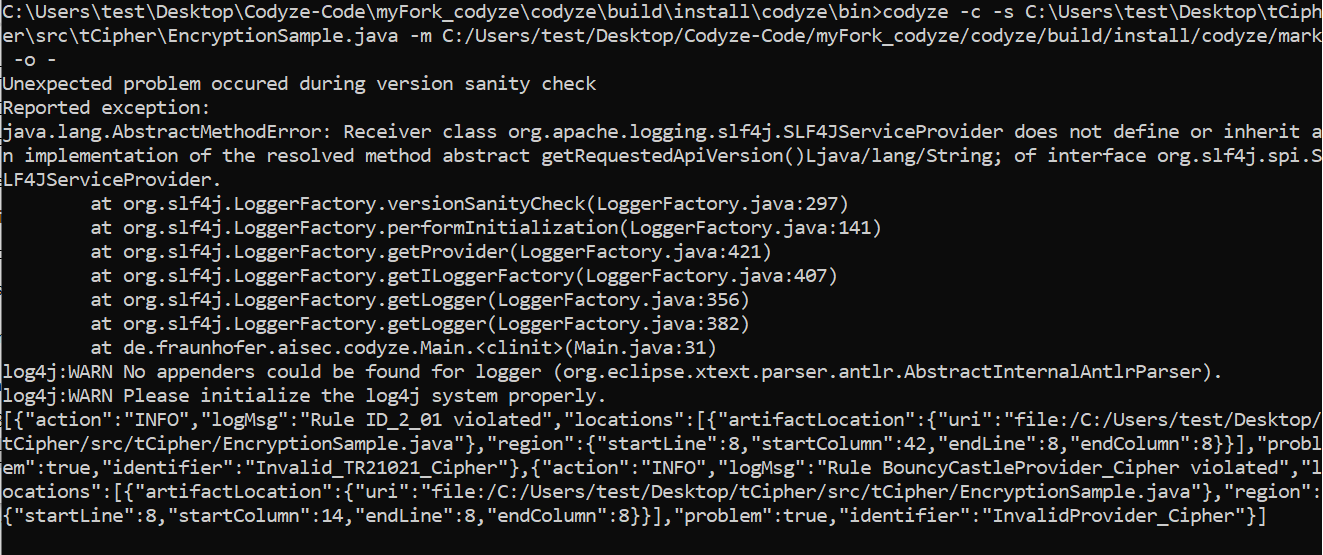
\includegraphics[width=1\linewidth]{thesis/figures/codyzecommand.PNG}
\caption{Result of the analysis of Listing \ref{lst:codesample} by \codyze{} in command-line.}
\label{fig:codyzecl}
\end{figure}

\cognicrypt's plugin provides toolbar and context menu buttons for triggering \cognicryptsast{} and \cognicryptgen{}. Moreover, it provides an option to only analyze the dependencies of a project. Figure \ref{fig:cccl} shows the result of the analysis done by \cognicryptsast{} in command-line. This analysis identified a Constraint error, indicating that the Cipher algorithm was insecure and a RequiredPredicate error, indicating that the key used in the Cipher has not been generated with a proper key generator API. The Figure \ref{fig:cccl} displays the name of the class and the method in which the error occurs. Thereafter, the type of error and the violated rule are displayed. This is followed by the error message and the statement that contains the error. The description of an error generated by \cognicryptsast{} on the command-line and in the Eclipse IDE are similar. 
\begin{figure}[H]
\centering
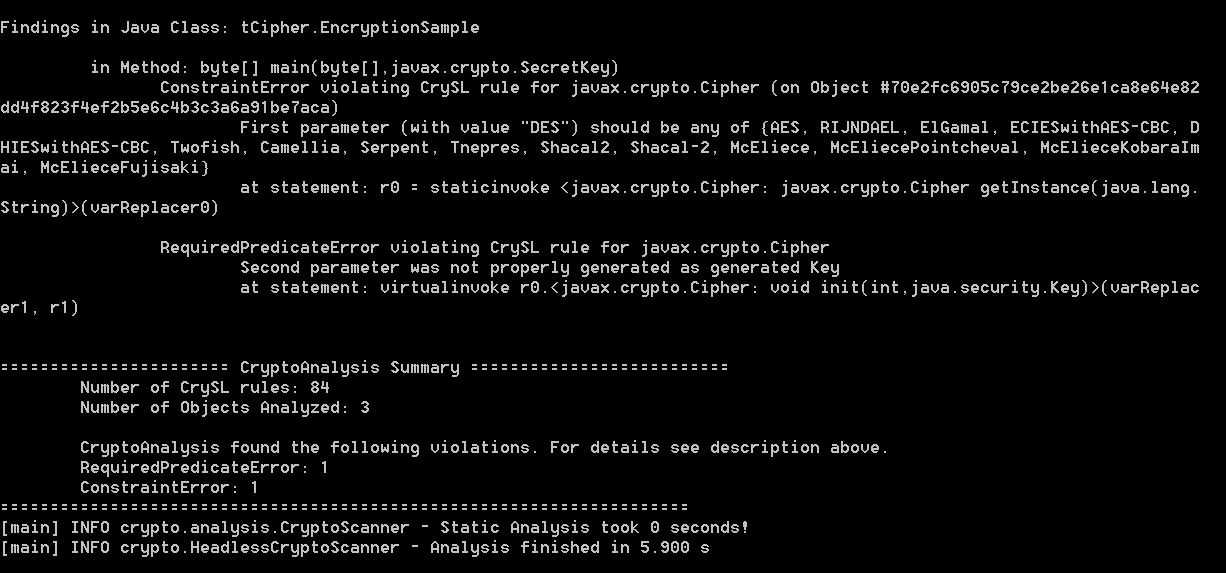
\includegraphics[width=1\linewidth]{thesis/figures/CCCommand.PNG}
\caption{Result of the analysis of Listing \ref{lst:codesample} by \cognicryptsast{} in command-line.}
\label{fig:cccl}
\end{figure}



\section{DSL Comparison}
\label{sec:dsl}
\crysl{} \cite{skm19} and \MARK{} \cite{cod} are the DSLs used by \cognicryptsast{} \cite{skm19} and \codyze{} \cite{cod}, respectively, to specify the correct usages of cryptographic APIs. 
This section aims to compare the DSLs on a theoretical and practical level fairly. Therefore, we performed a systematic review \cite{systematic4} of ways to compare DSLs. We searched on different platforms like Google\footnote{https://www.google.com}, GoogleScholar\footnote{https://scholar.google.com}, IEEE explore digital library\footnote{https://ieeexplore.ieee.org}, and ResearchGate\footnote{https://www.researchgate.net} for related articles and read the relevant ones, but there is no publication that compares DSLs in the same domain in terms of expressiveness. Rather, we found similar yet unrelated papers. For example, Cuadrado \etal{} compared two DSLs with the same syntax but different implementation techniques (internal and external) in their paper \cite{evaldsl14}. But that is not suitable for our DSLs since \MARK{} and \crysl{} are both external DSLs and this comparison is not useful. The other papers discussed comparing DSLs and GPLs (General Purpose Languages) to test program comprehension via user studies, which is not the focus of our study \cite{dslvsgpl12} or measuring usage simplicity in DSLs and GPLs \cite{empdslvsgpl10}, or comparisons of ways to define DSLs \cite{comptext8}, which are all unrelated to our research. Several studies tested usability \cite{usabil12} \cite{usabledsl11} \cite{qualitydsl11} \cite{successfac09}, which requires a user study and is beyond the scope of this thesis.

Thus, we propose translating \crysl{} rules to \MARK{} rules, and vice versa, to explore their expressiveness.
By translating one language to another and vice versa in a particular domain, such as defining correct usages of cryptographic APIs, we are expressing elements of one language in another while preserving the meaning, which demonstrates the expressiveness in that particular domain. There will be four possible scenarios in our case of translation. If we can translate \MARK{} rules into \crysl{} and \crysl{} rules into \MARK, then \MARK{} and \crysl{} are equally expressive when defining rules for cryptographic APIs.	However, if \crysl{} rules can be expressed by \MARK, but \MARK{} rules cannot be translated into \crysl, then \MARK{} is more expressive in specifying cryptographic API rules. Additionally, if \MARK{} rules could be expressed by \crysl{}, and \crysl{} rules could not be expressed by \MARK{}, then \crysl{} is more expressive than \MARK{} in defining rules for cryptographic APIs. Finally, if \crysl{} rules and \MARK{} rules cannot be translated into each other, then they express different things in defining rules for cryptographic APIs. 


Prior to comparing the DSLs, we provide a short explanation of \MARK{} and \crysl. We will then compare them practically and translate the rules, and finally, we will compare them theoretically.

\subsection{\crysl{}}
\label{subsec:crysl}
\crysl{} is a domain-specific language (DSL) that allows cryptography experts to describe secure usage of their crypto APIs in a lightweight special-purpose syntax \cite{skm19}. The \crySL compiler is built upon Xtext \cite{xtext}, an open-source framework for developing domain-specific languages. Based on the \crysl{} grammar, Xtext provides parsing, type checking, and syntax highlighting capabilities. A \crysl{} rule is a simple text file and can be written in any text editor. Eclipse can be used to create \crysl{} rules with syntax correction by installing the \crysl{} editor. 

Currently, \crysl{} rules have been developed by crypto experts of \cognicrypt{} developers for JCA, Bouncy Castle \cite{bc}, a Java library that extends Java Cryptographic Extension (JCE)\footnote{JCE is an API that provides a framework that allows Java developers to implement security features \cite{jce}.}, Bouncy Castle JCA \cite{bc}, Bouncy Castle provider for the JCA, and Tink \cite{tk}, an open-source easy to use and secure cryptographic library made by Google to reduce API misuses \cite{apirules}.

A \crysl{} rule is written for each class and consists of 6 mandatory and 3 optional parts. We introduce the semantics of \crysl{} rules by using the \crysl{} rule for javax.crypto.KeyGenerator in Listing \ref{lst:orgkeygencrysl} as an example. We further use part of the \crysl{} rule for javax.crypto.spec.PBEKeySpec (Listing \ref{lst:orgpbecryslRule}) to elaborate some infrequently used terms.
\pagebreak
\begin{lstlisting}[language=crysl,caption= {KeyGenerator \crysl{} rule from JCA API \cite{apirules}}., label={lst:orgkeygencrysl}, escapechar=^]
SPEC javax.crypto.KeyGenerator ^\label{line:spec}^

OBJECTS
	int keysize; ^\label{line:objects1}^
	java.security.spec.AlgorithmParameterSpec params;
	javax.crypto.SecretKey key;
	java.lang.String algorithm;
	java.security.SecureRandom random;^\label{line:objects2}^

EVENTS
	g1: getInstance(algorithm);^\label{line:g1}^
	g2: getInstance(algorithm, _); ^\label{line:g2}^
	Get := g1 | g2; ^\label{line:get}^

	i1: init(keysize); ^\label{line:i1}^
	i2: init(keysize, random);
	i3: init(params);
	i4: init(params, random);
	i5: init(random); ^\label{line:i2}^
	Init := i1 | i2 | i3 | i4 | i5;
    
	gk1: key = generateKey(); ^\label{line:gk1}^
	GenKey := gk1; ^\label{line:genkey}^

ORDER
	Get, Init?, GenKey ^\label{line:ordercrysl}^

CONSTRAINTS
	algorithm in {"AES", "HmacSHA256", "HmacSHA384", "HmacSHA512"};^\label{line:const1}^
	algorithm in {"AES"} => keysize in {128, 192, 256};^\label{line:const2}^
   
REQUIRES
	randomized[random]; ^\label{line:requirerandom}^
    
ENSURES 
	generatedKey[key, algorithm]; ^\label{line:generatedkey}^
\end{lstlisting}


\subsubsection{Mandatory sections}
On the first line (\ref{line:spec}), there is SPEC that indicates the class name. The OBJECTS (Line \ref{line:objects1} to \ref{line:objects1}) are parameters or return values of methods in the EVENTS section. All methods that may contribute to the successful use of an object of the \crysl{} rule are described in the EVENTS section. Each method pattern is represented by a label in the EVENTS section (e.g., \code{Get} in Line \ref{line:get}). When different patterns of the same method are possible, only one of them based on the implementation will be chosen in the ORDER section. For example, in Listing \ref{lst:orgkeygencrysl} Lines \ref{line:g1} and \ref{line:g2} show two patterns of \code{getInstance} method: \code{g1} with only one parameter, and \code{g2} with two parameters. \crysl{} uses aggregates to represent the disjunction of labels (e.g., \code{Get} in line \ref{line:get}).

The ORDER section defines a usage pattern in the form of regular expression for methods in the EVENTS section. An example would be the \code{getInstance} call (Line~\ref{line:ordercrysl}) followed by the \code{init} call (which is optional), followed by a call to the \code{generateKey} method in Listing \ref{lst:orgkeygencrysl}.

The CONSTRAINTS show constraints for objects. For instance, Line~\ref{line:const1} maintains that \code{algorithm} must be one of the following: AES, HmacSHA256, HmacSHA384, HmacSHA512. The Line \ref{line:const2} indicates that if the \code{algorithm} is AES, then the \code{keySize} must be one of 128, 192, or 256.
 
Assuming that the object is used appropriately, meaning that all limitations in the CONSTRAINTS section and usage patterns in the ORDER section are considered, the ENSURES section defines what a class predicates. Line \ref{line:generatedkey} of the keyGenerator \crysl rule demonstrates that using this class properly ensures the generation of a \code{key} with a specific \code{algorithm}.
  
\crysl{} allows us to define a method-event pattern using the \emph{after} keyword (Line~\ref{line:enskey}). For example, in Line~\ref{line:enskey} of Listing \ref{lst:orgpbecryslRule}, \code{speccedKey} predicate is created if the appropriate method is called. Thus, the PBEKeySpec class ensures the generation of a key after a call to the appropriate constructor with a specified \code{keyLength}.

 

\begin{lstlisting}[language= CrySL,caption= Part of \crysl{} rule for javax.crypto.spec.PBEKeySpec from JCA ruleset \cite{apirules}., label={lst:orgpbecryslRule}, escapechar=|]
SPEC javax.crypto.spec.PBEKeySpec

OBJECTS
    ...
FORBIDDEN
	PBEKeySpec(char[]) => Con; |\label{line:forbidden1}|
	PBEKeySpec(char[],byte[],int) => Con; |\label{line:forbidden2}|
	
EVENTS
	Con: PBEKeySpec(password, salt, iterationCount, keyLength); |\label{line:eventcon}|
	
	ClearPass: clearPassword();|\label{line:clearpass}|
...
CONSTRAINTS
	iterationCount >= 10000;
	neverTypeOf[password, java.lang.String]; |\label{line:nevertyp}|
	notHardCoded[password]; |\label{line:nothardcod}|
...
ENSURES
	speccedKey[this, keyLength] after Con; |\label{line:enskey}|
	
NEGATES
	speccedKey[this, _] after ClearPass; |\label{line:neg}|
\end{lstlisting}


\subsubsection{Optional sections}
Apart from mandatory sections that each \crysl{} rule must have, some \crysl{} rules may contain optional sections. The FORBIDDEN section involves calls to the methods that are insecure. The PBEkeySpec constructor call must consume a salt to generate a more secure key, whereas the signatures of the constructors in Lines~\ref{line:forbidden1} and~\ref{line:forbidden2} do not consume a salt; therefore, those calls are insecure and forbidden. After the \code{clearPassword} call, a PBEKeySpec object made by a constructor is no longer valid. \crysl{} allows invalidating a current predicate in the NEGATES field. As shown in Line~\ref{line:neg}, after \code{clearPassword} is called, the PBEkeySpec object is no longer effective. The predicates that one rule ENSURES can be used in the REQUIRES section of another rule. For example, Line~\ref{line:requirerandom} requires that the salt be generated from a random seed.


\crysl{} developers have added some simple built-in auxiliary functions to make it more expressive. For example, in Listing \ref{lst:orgpbecryslRule}, the function
\code{neverTypeOf} in Line \ref{line:nevertyp} states that the password should never be of type \code{String} and Line \ref{line:nothardcod} states that the password should not be hard-coded. \cite{stefanphd} fully described all of the built-ins in \crysl.
\subsection{\MARK{}}
\label{subsec:mark}
\MARK{} is a domain-specific language for writing rules to specify the correct usage patterns of APIs or libraries \cite{cod}. It stands for "Modellierungssprache fuer Anforderungen und Richtlinien der Kryptografie" (Modeling Language for Cryptography Requirements and Guidelines). \MARK{}'s grammar is written using Xtext. \MARK{}'s Eclipse plugin project \cite{markgithub} provides several features for \MARK{} language, including a language server for using \MARK{} in IDEs with LSP support, an Xtext generator that creates Crymlin/Gremlin from \MARK{} files, and an Eclipse plugin for syntax highlighting, auto-completion, and code correction \cite{markgithub}. Unfortunately, there are no further details available regarding the use of \MARK{} on other IDEs with LSP support or the creation of Crymlin/Gremlin out of \MARK{} files. In order to fully grasp these concepts, it is necessary to conduct extensive research on the implementation of \MARK{}, which is beyond the scope of this thesis.

Currently, there are \MARK{} policies made by \codyze's developers for the Botan \cite{botan}, a C++ cryptography library, Bouncy Castle and Jackson \cite{jackson}, a high-performance JSON processor for Java libraries for cryptography in Java. After reviewing the \MARK{} ruleset on \codyze's Github page, we discovered that the Bouncy Castle \MARK{} ruleset contains rules for the JCA API. However, we will continue to refer to it as the Bouncy Castle \MARK{} ruleset.

Writing \MARK{} rules for a library necessitates a thorough knowledge of the API and class structure of the library. \MARK{} policies are separated into two parts that we will discuss in separate sections; Entities (see Section \ref{subsubsec:entity}) and Rules (see Section \ref{subsubsec:rule}). Rules determine the correct usage of the entities. Entities are an abstract grouping of API functions. Entity contains three parts:
\begin{itemize}
\item \emph{Name}, the name of the rule.
\item \emph{Ops}, set of operations (op).
\item \emph{Var}, variables that refer to function arguments or return values.
\end{itemize}


Here we will provide a brief overview of the entity and rule parts of \MARK{} policies.

\subsubsection{Entity}
\label{subsubsec:entity}
To describe entities, we consider Listing \ref{lst:orgkeygenmarken} which shows the entity part of the \MARK{} policy for javax.crypto.KeyGenerator and Listing \ref{lst:orgsecureRandomMARK} which is a part of \MARK{} entity file for java.security.SecureRandom to describe a less frequently used optional keyword, \code{forbidden}, in \MARK{}.

\begin{lstlisting}[language=MARK,caption= {\MARK{} entities for javax.crypto.KeyGenerator of Bouncy Castle ruleset \cite{codyzegit}}, label={lst:orgkeygenmarken}, escapechar=@]
package java.jca

entity KeyGenerator {
    
    var algorithm;@\label{line:varsbeg}@
    var provider;
    
    var keysize;
    var random;
    var params;
    var key;@\label{line:varsend}@
    
    op instantiate {@\label{line:opsbeg}@
        javax.crypto.KeyGenerator.getInstance(algorithm : java.lang.String); @\label{line:instance1}@
        javax.crypto.KeyGenerator.getInstance(@\label{line:instance2}@
            algorithm : java.lang.String,
            provider : java.lang.String | java.security.Provider
        );
    }
    
    op init {
        javax.crypto.KeyGenerator.init(keysize : int);
        javax.crypto.KeyGenerator.init(
            keysize : int,
            random : java.security.SecureRandom
        );
        javax.crypto.KeyGenerator.init(random : java.security.SecureRandom);
        javax.crypto.KeyGenerator.init(params : java.security.spec.AlgorithmParameterSpecs);
        javax.crypto.KeyGenerator.init(
            params : java.security.spec.AlgorithmParameterSpec,
            random : java.security.SecureRandom
        );
    }
    
    op generate {
        key = javax.crypto.KeyGenerator.generateKey();
    }@\label{line:opsend}@
}
\end{lstlisting}

The first step is to define model relevant classes as \MARK{} entities. Only those classes which contain the relevant data or function must be identified as \MARK{} entities. Even though many programming languages classes can be combined in an abstract \MARK{} entity in several cases, it can at first be easier to map classes explicitly into entities. For instance, KeyGenerator class to entity KeyGenerator. Developers can freely choose the name of the entity \cite{cod}.

The second step is to define ops and variables. An op is a semantically equivalent or related group of functions, methods, or constructors, provided as completely qualified signatures. The most common ops in cryptographic libraries are, instantiate, initialize, update, finalize and reset. For example, in Listing \ref{lst:orgkeygenmarken}, we have instantiate op, which shows the \code{getInstance} methods with different possible parameters (Lines~\ref{line:instance1},~\ref{line:instance2}). The type of each op's parameters with a name is specified, but we can also have unnamed and untyped parameters (described with "\_"). These parameters do not play any role in the definition of rules. Named parameters must also be declared as entity variables using the \code{var} keyword (Lines~\ref{line:varsbeg} to~\ref{line:varsend}) \cite{cod}.

The third step, which is optional, is to blacklist the forbidden ops. In some cases, functions that are deprecated or established to be insecure should not be used in the program. The \code{forbidden} keyword in \MARK{} indicates that the use of the following functions is insecure. For example, Lines~\ref{line:forbidpbe1} and~\ref{line:forbidpbe2} of Listing \ref{lst:orgsecureRandomMARK} are forbidden calls when using the SecureRandom class because they do not respect Bouncy Castle as a provider \cite{cod}.

\begin{lstlisting}[language=MARK,caption= Part of \MARK{} entities for java.security.SecureRandom from Bouncy Castle ruleset \cite{codyzegit}., label={lst:orgsecureRandomMARK}, escapechar=^]
    ...
     op instantiate {
        ...
        java.security.SecureRandom.getInstanceStrong();
        
        // forbidden calls because they don't respect BC as provider
        forbidden java.security.SecureRandom(); ^\label{line:forbidpbe1}^
        forbidden java.security.SecureRandom(^\label{line:forbidpbe2}^
            seed : byte[]
        );
    }
    ...
\end{lstlisting}


\subsubsection{Rule}
\label{subsubsec:rule}
After defining entities, we can start writing rules. \MARK{} rules apply to instances of entities and specify the conditions that must be met in these instances. Instances of \MARK{} may correspond to actual objects but might also be abstract functions or variables in non-object-oriented languages and static methods. Listing \ref{lst:orgkeygenMARKrule} displays one of the \MARK{} rules associated with the KeyGenerator class from the Bouncy Castle \MARK{} files included in \codyze's Github repository.

Every rule has a unique name across all \MARK{} files loaded into \codyze{} (Line \ref{line:rulename}). \code{Using} keyword (Line \ref{line:usingpart}) initiates the declaration of instances of the \MARK{} entities, here KeyGenerator and javax.crypto.Mac instances, and \code{ensure} shows the condition (Line \ref{line:ensurepart}). A violation of the condition will result in a finding with a message indicated by the \code{onfail} identifier (Line \ref{line:onfail}). 


In some rules, some preconditions must be met before the main condition is evaluated. If they fail, the main condition will not be evaluated, and the rule will not return any results. Preconditions are declared by the \code{when} keyword (Line \ref{line:whenpart}). Mark includes several built-in functions that can be used as predicates in conditions and preconditions (e.g., Line \ref{line:builtinmark}). They are called during MARK rule evaluation and operate over their input arguments (usually MARK objects or constants) and the evaluation context. By convention, built-ins should begin with "\_". If a built-in fails, it will return an Error object which evaluates to not applicable, i.e., neither true nor false. 

In the following rule example (Listing \ref{lst:orgkeygenMARKrule}), once the preconditions are satisfied, i.e., if the Mac algorithm is AESCMAC (Line \ref{line:whencond}), and the variable Mac key equals the KeyGenerator key (Line \ref{line:builtinmark}), then the rule condition must be met, that is, the KeyGenerator's key must be greater than or equal to 128 (Line \ref{line:condition2}). Otherwise, the InsufficientCMACKeyLength error will be thrown.

\begin{lstlisting}[language=MARK2,caption= A \MARK{} rule associated with javax.crypto.KeyGenerator class from Bouncy Castle ruleset \cite{codyzegit}., label={lst:orgkeygenMARKrule}, escapechar=^]
rule ID_5_3_02_CMAC_Keygen {  ^\label{line:rulename}^
    using ^\label{line:usingpart}^
        Mac as m,
        KeyGenerator as kg
    when ^\label{line:whenpart}^
        m.algorithm in ["AESCMAC"] ^\label{line:whencond}^
        && _is(m.key, kg.key) ^\label{line:builtinmark}^
    ensure ^\label{line:ensurepart}^
        _is(m.key, kg.key) ^\label{line:condition1}^
        && kg.keysize >= 128 ^\label{line:condition2}^
    onfail  ^\label{line:onfail}^
        InsufficientCMACKeyLength 
}
\end{lstlisting}

In this example, the condition \code{\_is(m.key, kg.key)} is mentioned in both the \code{when} and \code{ensure} sections. It might be a mistake since if it is true in the \code{when} section, then it is also true in the \code{ensure} section, so there is no need to verify it again. The developers of \codyze{} did not elaborate on the matter further; therefore, we have opened an issue on \codyze{}'s Github repository\footnote{https://github.com/Fraunhofer-AISEC/codyze/issues/400}.

 

\subsection{Practical comparison of \crysl{} and \MARK{}}
\label{sec:practicdsl}

This section aims to compare the DSLs on a practical level. In order to accomplish this, we proposed translating \crysl{} rules to \MARK{} and vice versa. Since there are \MARK{} and \crysl{} rules for the Bouncy Castle JCA API for Java, we first translate Bouncy Castle JCA rules from \crysl{} to \MARK{} and vice versa. As stated before, there are no \MARK{} rules specified for the JCA library, which is the primary cryptography API for Java applications \cite{snb16}. In this regard, it is worthwhile to translate \crysl{} JCA rules in \MARK{} language and compare their functionality and result of their analyses on the same Java cryptography examples. So at the end we will have three translations, \crysl{} Bouncy Castle JCA to \MARK, \MARK{} Bouncy Castle JCA to \crysl{} and \crysl{} JCA to \MARK. Source codes for the translated rules are available in Appendices \ref{appendix:ruletranslaions}.

We developed the following translation based on the information we obtained from reviewing existing \MARK{} and \crysl{} rules, \crysl{} paper \cite{skm19} and \codyze's documentation page \cite{cod}. We will employ these translated rules in the evaluation of \codyze{} and \cognicryptsast{} (cf. Chapter \ref{ch:eval}).



\subsubsection{Setup}
\label{sec:rulesetup}
We used the same virtual machines we explained in Section \ref{sec:practical} to translate rules. On the first machine with Java 8, we installed the \crysl{} Eclipse plugin and on the second machine with Java 11, we installed the \MARK{} Eclipse plugin. We used the \crysl{} rules from the Crypto-API-rules Github repository master branch \cite{apirules} to the commit 1dbad34\footnote{\url{https://github.com/CROSSINGTUD/Crypto-API-Rules/commit/1dbad342a46c47df62e891fc25f46944972d9e18}} and \MARK{} rules from \codyze{} Github repository main branch \cite{codyzegit} to the commit 8c74a13\footnote{\url{https://github.com/Fraunhofer-AISEC/codyze/commit/8c74a13be2385b79875990c5e36ed67b39579662}}, to the date of October 31st, 2021.



\subsubsection{Translation from \crysl{} to \MARK{}}
There are 47 Bouncy Castle JCA and 49 JCA \crysl{} rules on Github \cite{apirules}. Each \crysl{} rule represents a class. While translating each rule to \MARK{}, we put entities (ops and vars) in one file and the rules on another file. As an example, there are two \MARK{} files for the KeyGenerator class, the KeyGenerator.mark file containing the entities of the class (see Listing \ref{lst:keygenmarkentrans}), and the Rule\_KeyGenerator.mark file containing the rules, such as order, constraints, etc (see Listing \ref{lst:keygenmarkruletrans}). Listings \ref{lst:keygenmarkentrans} and \ref{lst:keygenmarkruletrans} show KeyGenerator \MARK{} rule translated from its \crysl{} rule from JCA API in Listing \ref{lst:orgkeygencrysl} \cite{apirules}.

The objects (Lines \ref{line:objects1} to \ref{line:objects2}) of the \crysl{} rules (Listing \ref{lst:orgkeygencrysl}) are directly translated to vars (Lines \ref{line:var1} to \ref{line:var2}). \MARK{} variables are not typed. The type of variables will be specified in the ops. As an example, in \crysl{} the type of \code{keySize} is \code{int}. In translation to \MARK{}, the type of \code{keysize} is specified in the operation where it is being used (Line \ref{line:keysizetype}). Return variables will not be typed in \MARK{} (Line \ref{line:notypekey}). Furthermore, the functions in the EVENTS section have exactly the same translation and grouping in the corresponding \MARK{} rule (Lines \ref{line:op1} to \ref{line:op3end}) without any labels. We have three kinds of operations in this case, instantiate (Line \ref{line:op1}) for \code{getInstance} methods, init (Line \ref{line:op2}) for \code{init} methods and generate (Line \ref{line:op3}) for \code{generateKey} method.
\pagebreak

\begin{lstlisting}[language=MARK,caption=  {Entity part of translated KeyGenerator \crysl{} rule to \MARK{} from JCA API.}, label={lst:keygenmarkentrans}, escapechar=|]
package java.jca

entity KeyGenerator {
    
    var keySize;|\label{line:var1}|
    var params;
    var key;
    var algorithm;
    var random;|\label{line:var2}|
    
    op instantiate {|\label{line:op1}|
        javax.crypto.KeyGenerator.getInstance(algorithm : java.lang.String);
        javax.crypto.KeyGenerator.getInstance(
            algorithm : java.lang.String,
            _
        );
    }
    
    op init {|\label{line:op2}|
        javax.crypto.KeyGenerator.init(keySize : int);
        javax.crypto.KeyGenerator.init(
            keySize : int, |\label{line:keysizetype}|
            random : java.security.SecureRandom
        );
        javax.crypto.KeyGenerator.init(random : java.security.SecureRandom);
        javax.crypto.KeyGenerator.init(params : java.security.spec.AlgorithmParameterSpecs);
        javax.crypto.KeyGenerator.init(
            params : java.security.spec.AlgorithmParameterSpec,
            random : java.security.SecureRandom
        );
    }
    
    op generate {|\label{line:op3}|
        key = javax.crypto.KeyGenerator.generateKey(); |\label{line:notypekey}|
    }|\label{line:op3end}|
}
\end{lstlisting}

Listing \ref{lst:keygenmarkruletrans} shows the translated rules from ORDER, CONSTRAINTS, and REQUIRES sections of the KeyGenerator \crysl{} rule. The translation of \crysl{} ORDER section is the first rule in Listing \ref{lst:keygenmarkruletrans} Line \ref{line:ordermark}, which uses the same regular expression as the \crysl{} rule (Line \ref{line:ordercrysl}). The CONSTRAINTS in \crysl{} rule are the constraints over the \code{algorithm} and the \code{keysize} (Lines \ref{line:const1} and \ref{line:const2}) which direct translations are the second (Line \ref{line:algo}) and third (Line \ref{line:keysizemark}) rules of Listing \ref{lst:keygenmarkruletrans}. \MARK's analyzer checks all the rules, and if the ensure part is violated, an error is thrown even if the class has not been used in the analyzed project. We avoided this mistake by adding a when clause to all the \MARK{} rules (except the order rules) to determine if a variable corresponding to that rule exists, using the built-in method \code{\_has\_value}. The rule should not be tested if the variable is not present. The built-in function \code{\_has\_value(a)} checks whether a given \MARK{} variable, \code{a}, has a CPG-node which indicates that it exists as part of the program \cite{codyzegit}. In the Line \ref{line:hasvalue}, for instance, the analyzer checks whether the KeyGenerator's \code{algorithm} variable is present; otherwise, this rule is not executed.
 \pagebreak
\begin{lstlisting}[language=MARK2,caption= {Rule part of translated KeyGenerator \crysl{} rule to \MARK{} from JCA API.}, label={lst:keygenmarkruletrans}, escapechar=|]
package java.jca

rule JCAProvider_KeyGenerator_order{|\label{line:ordermark}|
	using
		KeyGenerator as kg
	ensure
		order
			kg.instantiate(),
			kg.init()?,
			kg.generate()
	onfail
		InvalidOrderOfKeyGenerator
}
//constraints
rule JCAProvider_KeyGenerator_algorithm{|\label{line:algo}|
	using
		KeyGenerator as kg
	when 
		_has_value(kg.algorithm)|\label{line:hasvalue}|
	ensure
		kg.algorithm in ["AES", "HmacSHA224", "HmacSHA256", "HmacSHA384", "HmacSHA512"]
	onfail
		InvalidSecretKeyAlgorithmOfKeyGenerator
}
rule JCAProvider_KeyGenerator_keysize{|\label{line:keysizemark}|
	using
		KeyGenerator as kg
	when
		kg.algorithm in ["AES"] && _has_value(kg.keySize)
	ensure
		kg.keySize in [128, 192, 256]
	onfail
		InvalidKeySizeOfKeyGenerator
}
//requires
rule JCAProvider_KeyGenerator_randomized{
	using
		KeyGenerator as kg,
		SecureRandom as sr
	when
		_has_value(kg.random)
	ensure
		_is(kg.random, sr)
	onfail
		NotRandomranGenOfKeyGenerator
}
\end{lstlisting}

The ENSURES and REQUIRES sections of \crysl{} bind two rules together, so when we translate them to \MARK, we include all classes that contain the same predicate in the REQUIRES and ENSURES sections of their \crysl{} rule as instances of the corresponding \MARK{} rule. We have placed the translation for this binding in the \MARK{} rule file of the class which used this predicate in its REQUIRES section. For instance, KeyGenerator \crysl{} rule ENSURES \code{generatedKey[key, algorithm]} (Line \ref{line:generatedkey}) which means if the KeyGenerator is used properly, then it guarantees a key with the corresponding algorithm.


This predicate appears in the Mac\footnote{https://github.com/CROSSINGTUD/Crypto-API-Rules/blob/master/BouncyCastle-JCA/src/Mac.crysl} and Cipher\footnote{https://github.com/CROSSINGTUD/Crypto-API-Rules/blob/master/BouncyCastle-JCA/src/Cipher.crysl} \crysl{} rule's REQUIRES section, so the \MARK{} rules are placed within the Mac and Cipher \MARK{} rule files.

Listing \ref{lst:macmarkruletrans} illustrates the translation of the \code{generatedKey} predicate in the Mac \MARK{} rule file. The Mac \crysl{} rule specifies this predicate as \code{generatedKey[key, \_]} in its REUIRES section. This predicate indicates that the key variable used in creating the Mac instance must be generated appropriately using KeyGenerator or any other rule that has \code{generatedkey[javax.crypto.SecretKey,java.lang.String]} in their ENSURES section. The second parameter in the predicate, \code{generatedKey[key,\_]}, is an underscore, which implies that the algorithm used to generate the key does not matter.


As well as KeyGenerator, there are other rules in \crysl{} that guarantee this predicate, such as SecretKeySpec, KeyStore and SecretKeyFactory. Therefore, we include all of them as instances in the Mac \MARK{} rule (Line \ref{line:seckey1} to \ref{line:seckey2}).
 
We then provide a precondition to guarantee the existence of the Mac instance by checking that a key variable for this instance exists in the program (Line \ref{line:keyhasvalue}). 

According to the Mac \crysl{} rule, it does not matter what algorithm is being used to generate the key, therefore, we only need to confirm that the key is generated by one of the mentioned classes. To accomplish this, we use the built-in function \code{\_is} (Line \ref{line:ensurekeys}). The built-in \code{\_is(a,b)} checks if two objects are equal \cite{codyzegit}. InvalidGeneratedKeyOfMac error message on Line \ref{line:errormessage} may appear if the program does not conform to this rule. 
 
\begin{lstlisting}[language=MARK2,caption= {Part of translated Mac \crysl{} rule to \MARK{} from JCA API.}, label={lst:macmarkruletrans}, escapechar=@]
rule JCAProvider_Mac_generatedkey{
	using
		Mac as m,
		KeyStore as ks, @\label{line:seckey1}@
		SecretKeyFactory as skf,
		KeyGenerator as kg,
		SecretKeySpec as sks @\label{line:seckey2}@
	when 
	    _has_value(m.key) @\label{line:keyhasvalue}@
	ensure
		_is(m.key, sks) || _is(m.key, skf.key)|| _is(m.key, kg.key) || _is(m.key, ks.key) @\label{line:ensurekeys}@
	onfail
		InvalidGeneratedKeyOfMac @\label{line:errormessage}@
}
\end{lstlisting}

In \crysl{} it is possible to specify a method-event pattern using
the keyword \emph{after}. For example, in Listing \ref{lst:orgpbecryslRule} of PBEKeySpec \crysl{} rule, we have the following predicate: \code{speccedKey[this, \_] after ClearPass} (Line \ref{line:neg}), which indicates that after using the \code{clearPassword} method, the speccedkey generated by PBEKeySpec is no longer valid. Since \MARK{} does not provide this feature, it is not possible to translate the NEGATES section of the \crysl{} rules to \MARK.


We can define forbidden methods in \MARK, which is equivalent to the FORBIDDEN section of the \crysl{} rules. The forbidden methods are located in the entity part of the \MARK{} rule. Listing \ref{lst:pbekmarkentrans} shows a part of the translation of the PBEKeySpec \crysl{} rule to \MARK{} entities. Lines \ref{line:forbid1} and \ref{line:forbid2} show the translation of the FORBIDDEN section of PBEKeySpec \crysl{} rule (Lines \ref{line:forbidden1} and \ref{line:forbidden2}) to \MARK. These lines forbid the use of the PBEKeySpec method with 1 or 3 parameters; in another way, the method PBEKeySpec should only be used with four parameters; otherwise, it is considered insecure.


\begin{lstlisting}[language=MARK,caption= {Part of Entity part of translated PBEKeySpec \crysl{} rule to \MARK{} from JCA API.}, label={lst:pbekmarkentrans}, escapechar=|]
package java.jca

entity PBEKeySpec {
    ...
	op instantiate {

		javax.crypto.spec.PBEKeySpec(
			password : char[],
			salt : byte[],
			iterationCount : int,
			keyLength : int
		);
		forbidden javax.crypto.spec.PBEKeySpec(_: char[]);|\label{line:forbid1}|
		forbidden javax.crypto.spec.PBEKeySpec(_: char[],_: byte[],_: int);|\label{line:forbid2}|
	}
    ...
}
\end{lstlisting}

\subsubsection*{Discussion}
\crysl{}'s compiler provided auto-completion, syntax checking, and case sensitivity. During the translation of \crysl{} rules into \MARK{}, some language features could not be translated. There is, for example, no such method in \MARK{} where we can retrieve an element of an array. There is \code{elements} in \crysl, but no equivalent method in \MARK. However, this is not a significant issue because this method can easily be added as a built-in method in \MARK. The same holds true for other built-in functions as well, such as noCallTo, callTo. The three built-in functions, \code{mode}, \code{alg}, and \cod{padding} are available via \code{\_split} in \MARK.

There is a keyword, \code{after} that has been used in the sections REQUIRES, ENSURES, and NEGATES. This keyword cannot be translated into \MARK{} since there is no equivalent feature to \code{after} in \MARK. Moreover, we cannot include method calls in conditions or preconditions. In such cases, we translated the rules without considering the \code{after} part. For instance, the Line \ref{line:enskey} in Listing \ref{lst:orgpbecryslRule} ensures that a speccedKey with a certain keyLength is generated after a call to the constructor specified in the EVENTS section. This rule was translated without translating the \code{after} keyword, which is reasonable since the constructor call is the final and only call in the order section and will be called when generating a PBEKeySpec instance. When the method following the keyword \code{after} is not a final method, the rules are not equal, and the \MARK{} translation is incomplete. Further, it is not possible to translate the NEGATES section of \crysl{} rules to \MARK, as there is no equivalent feature to \code{after} in \MARK{} and this section depends entirely on this keyword.
\label{sec:marktocrysl}

% \subsection{Translate Bouncy Castle JCA API from \MARK{} to \crysl{}}
% \input{thesis/chapters/4-comparison/bcmarktocrysl}

\subsubsection{Translation from \MARK{} to \crysl{}}
There are \MARK{} rules for 60 classes Bouncy Castle JCA API on Github\footnote{https://github.com/Fraunhofer-AISEC/codyze/tree/main/src/dist/mark}. However, we could only translate 57 of them cause three classes require Java 9 or higher versions, which are javax.crypto.spec.ChaCha20ParameterSpec, java.security.spec.XECPrivateKeySpec and java.\-security.SecureRandomParameters. Our first step was to translate \MARK{} entities to \crysl, then we added the written \MARK{} rules from rule files to the \crysl{} rules. In \MARK, interfaces, such as PrivateKey and PublicKey, should also be added, as a rule; otherwise, they are not recognized by \MARK. The same is not true in \crysl, but we translated them too as a matter of fairness.

The vars (Lines \ref{line:varsbeg} to \ref{line:varsend}) and ops (Lines \ref{line:opsbeg} to \ref{line:opsbeg}) of KeyGenerator entity \MARK{} file in Listing \ref{lst:orgkeygenmarken} translate to OBJECTS and EVENTS in \crysl. Listing \ref{lst:transkeygencrysl} shows the KeyGenerator \crysl{} rule that is translated from the \MARK{} rule. OBJECTS and EVENTS are shown on Lines \ref{line:OBJECTS} and \ref{line:EVENTS} respectively.
\pagebreak
\begin{lstlisting}[language= CrySL,caption= {Translated KeyGenerator \MARK{} rule\protect\footnotemark~to \crysl{} from Bouncy Castle JCA API.}, label={lst:transkeygencrysl}, escapechar=@]
SPEC javax.crypto.KeyGenerator
OBJECTS @\label{line:OBJECTS}@
	java.lang.String algorithm;
	java.security.Provider provider;
	java.lang.String providerS;
	int keySize;
	java.security.SecureRandom random;
	java.security.spec.AlgorithmParameterSpec params;
	javax.crypto.SecretKey key;
	
//FORBIDDEN
//	getInstance(algorithm) => Instances;

EVENTS @\label{line:EVENTS}@
	ins1 : getInstance(algorithm, provider);
	ins2 : getInstance(algorithm, providerS);
	//ins3 : getInstance(algorithm);@\label{line:noprovider}@
	Instances := ins1| ins2;@\label{line:agg}@
	
	i1 : init(keySize);
	i2 : init(keySize, random);
	i3 : init(random);
	i4 : init(params);
	i5 : init(params, random);
	Inits := i1| i2| i3| i4| i5;

	g : key = generateKey();
	GenK := g;
	
ORDER
	Instances?, Inits?, GenK? @\label{line:order}@

CONSTRAINTS
	providerS in {"BC"};@\label{line:BC}@
	instanceOf[provider, org.bouncycastle.jce.provider.BouncyCastleProvider];@\label{line:provider}@
	keySize >= 128; @\label{line:keysize}@

//REQUIRES
//*

ENSURES
	generatedKey[key];
	generatedKey[key, algorithm];
\end{lstlisting}
\footnotetext{\url{https://github.com/Fraunhofer-AISEC/codyze}}

There is no single file containing all the \MARK{} rules that are related to a single class in the Github. Among all the \MARK{} rule files for Bouncy Castle JCA API, there were four rules containing the KeyGenerator class (Listing \ref{lst:keygenmarkrules})

\begin{lstlisting}[language=MARK2,caption= {\MARK{} rules for KeyGenerator of Bouncy Castle JCA API.}, label={lst:keygenmarkrules}, escapechar=@]
rule BouncyCastleProvider_KeyGenerator { @\label{line:rule1}@
    using
        KeyGenerator as kg
    ensure 
        _has_value(kg.provider)
        && (
            kg.provider == "BC"
            || _is_instance(kg.provider, "org.bouncycastle.jce.provider.BouncyCastleProvider")
        )
    onfail
        InvalidProvider_KeyGenerator
}
rule ID_5_3_02_GMAC {@\label{line:rule2}@
    using
        Mac as m,
        KeyGenerator as kg,
        SecretKeySpec as sks,
        SecretKeyFactory as kf
    when
        m.algorithm in ["AES-GMAC"] && ( _is(m.key, kg.key)
        || ( _is(m.key, kf.outkey) && _is(kf.keyspec, sks) ) )
    ensure
        // find a keygenerator of sufficient size
        kg.keysize >= 128
        || (_has_value(sks.len) && sks.len >= 128)
        || (!(_has_value(sks.len)) && _has_value(sks.key) && _length(sks.key) >= 16)
    onfail
        InsufficientGMACKeyLength
}
rule ID_5_3_02_CMAC_Keygen {@\label{line:rule3}@
    using
        Mac as m,
        KeyGenerator as kg
    when
        m.algorithm in ["AESCMAC"]
        && _is(m.key, kg.key)
    ensure
        // find a keygenerator of sufficient size
        _is(m.key, kg.key)
        && kg.keysize >= 128
    onfail
        InsufficientCMACKeyLength
}

rule ID_5_3_02_HMAC_Keygen {@\label{line:rule4}@
    using
        Mac as m,
        KeyGenerator as kg
    when
        m.algorithm in ["HMACSHA256", "HMACSHA512/256", "HMACSHA384",@\label{line:algos}@ "HMACSHA512", "HMACSHA3-256", "HMACSHA3-384", "HMACSHA3-512"]
        && _is(m.key, kg.key)
    ensure
        // find a keygenerator of sufficient size
        (
            _is(m.key, kg.key)
            && kg.keysize >= 128 @\label{line:keysizemark}@
        )
        || (
             _is(m.key, kg.key)
             && kg.algorithm == m.algorithm
        )
    onfail
        InsufficientHMACKeyLength
        }
\end{lstlisting}


In order to avoid complexity, we will only explain the parts of the rule relevant to KeyGenerator, although the explanations apply to other parts, as well.

According to the first rule (Line \ref{line:rule1}), when using the KeyGenerator class, the \code{getInstance} method must pass the \code{provider} parameter, which should either be the string "BC" or of type org.bouncycastle.jce.provider.BouncyCastleProvider. Lines \ref{line:BC} and \ref{line:provider} of Listing \ref{lst:transkeygencrysl} present the translation of this rule, in which we define constraints on the variables, \code{providerS} and \code{provider}. Because the existence of a provider is required, we removed \code{getInstance} method patterns in the EVENTS section that did not include a provider as a parameter (Line \ref{line:noprovider}) and created an aggregation of the rest (Line \ref{line:agg}). Moreover, the first rule suggests that this pattern of \code{getInstance} method (Line \ref{line:noprovider}) should not be used, which implies that the usage of this pattern is forbidden. We therefore added this method pattern to the FORBIDDEN section, but an error occurred as there is an issue with the \crysl{} grammar that currently allows us only to add constructor calls to the FORBIDDEN section. As a result, we commented the FORBIDDEN section.
Unlike \crysl, a variable may have multiple types in \MARK, which is why the variable \code{provider} in \MARK{} is divided into two variables in \crysl, \code{provider} of type java.security.Provider, and \code{providerS} of type java.lang.String.

The second rule (Line \ref{line:rule2}) states that whenever a Mac object is used with the AES-GMAC algorithm and a key generated by the KeyGenerator, the \code{keySize} must be greater than or equal to 128. In \crysl{} we are not able to write such clauses with those premises; in other words, we cannot add constraints to a rule's OBJECTS from another rule.
The solution would be to make a constraint on that variable, \code{keySize}, in the CONSTRAINTS section of the KeyGenerator \crysl{} rule (Line \ref{line:keysize}). This solution is logical since BSI (Bundesamt Für Sicherheit in der Informatikstechnik) has demonstrated that a \code{keySize} less than 128 bits is considered insecure \cite{BSI}.

As indicated by the third rule (Line \ref{line:rule3}), if the Mac object is used with the AESCMAC algorithm and a key generated by KeyGenerator, \code{keySize} must be at least 128 bits. Translation of this rule is the same as for the second rule we previously translated.

If a Mac object uses the algorithms specified in the Line \ref{line:algos} of the fourth rule (Line \ref{line:rule4}), and the key was generated by KeyGenerator, then either the \code{keySize} should be greater than or equal to 128 or the algorithm used in Mac and KeyGenerator are the same. We have already implemented the first part in the second and third rules. However, for the second part of the rule, we added a predicate to the ENSURES section of the KeyGenerator rule that guarantees a key with a specific algorithm, and we used this predicate in the REQUIRES section of the Mac rule.

The \crysl{} language was designed to define a usage pattern for each rule in the ORDER section, even if the class only contains a constructor call. A rule will not function without a usage pattern. Therefore, we have included the order in a regular expression that includes all the aggregates from the EVENTS section in such a way that there is no correct order established (Line \ref{line:order}), except for the rules for which we had a defined order in the \MARK{} version. Thus, the translation of \MARK{} rules into \crysl{} may not be syntactically identical; however, they convey the same semantic information.


\subsubsection*{Discussion}
The \MARK{} compiler does not support some of the features that the documentation \cite{cod} describes. The language lacks case-sensitivity and auto-completion, and it does not recognize non-defined variables but provides syntax checking. In \MARK{} we have to write an entity file for every interface or class that we intend to use, even if there is only a package and entity name. For example, PrivateKey or PublicKey interfaces. The \MARK{} grammar can detect if a class used in a rule is not defined in the folder in which all \MARK{} rules are stored.

As mentioned previously, a variable of one class cannot be constrained by a rule of another class in \crysl. As a result, we had to add the constraint in the CONSTRAINTS section without considering the precondition, so the rule for \crysl{} was not exactly the same as the \MARK{} rule. For instance, the translation of the \MARK{} rule on Line \ref{line:keysizemark} of Listing \ref{lst:keygenmarkrules} is the Line \ref{line:keysize} in the \crysl{} rule in Listing \ref{lst:transkeygencrysl}. In some cases, there were different constraints for the same variables under different preconditions. For example, the constraint for the \code{tLen} (the authentication tag length) variable of the GCMParameterSpec (gcm) class are \code{gcm.tLen >= 64} and \code{gcm.tLen >= 96} in 2 different rules with different preconditions. Our solution was to add the conjunction (\code{gcm.tLen >= 96}).

\MARK{} and \crysl{} do not have fully equivalent built-in functions. The built-in functions \code{\_is\_instance}, and \code{\_length} in \MARK{} have the same functionality as \code{instanceOf}, and \code{length} in \crysl, respectively.
There are \MARK{} built-in functions that are not used in the current \MARK{} rules but are defined in the \codyze{} Github repository \cite{codyzegit}, namely: \code{\_direct\_eog\_connection}, \code{\_eog\_connection}, \code{\_inside\_same\_function}, \code{\_get\_code}, \code{\_now}, \code{\_receives\_value\_from}, \code{\_split\_disjoint}, \code{\_split\_match\_unordered}, \code{\_starts\_with}, \code{\_year} \cite{codyzegit}.



\label{sec:crysltomark}

\subsection{Theoretical comparison of \crysl{} and \MARK{}}
\label{sec:theodsl}

\MARK{} and \crysl{} DSLs are both designed to specify the correct use of cryptographic APIs. \crysl{} is intended to be used to write rules only for Java cryptographic APIs. Nevertheless, as we discussed in Section \ref{subsec:mark}, \MARK{} enables us to write rules for C and C++, as well as Java since the \MARK{} parser is designed to parse \MARK{} rules for C++ or C cryptographic APIs. 

The DSLs \MARK{} and \crysl{} are both external DSLs. Internal DSLs are those that are implemented within a general-purpose language as the host. An external DSL is a language that is parsed independently of the host \cite{dsl}. \crysl{} was designed specifically for cryptography experts and the existing \crysl{} rules were written by cryptography experts of the \crysl{} developers \cite{stefanphd}.
The current \MARK{} rules are based on the BSI \cite{BSI} TR-02102-1 version 2019-01
guideline for using cryptographic APIs.

\crysl{} and \MARK{} have different syntaxes; however, their semantics are similar in some cases, for example, vars in \MARK{} are equivalent to OBJECTS in \crysl, or ops are equivalent to EVENTS in \crysl. Since there is limited information about \MARK, we cannot be certain of similarities and differences in semantics. Therefore, we were required to perform a practical comparison in which we converted \MARK{} policies to \crysl{} and vice versa in Section \ref{sec:practicdsl}.

This also applies to the built-in functions. In order to determine how close we could get to expressing one language in another, we are required to ensure that each DSL contains sufficient built-in functions to enable us to translate rules written in the other DSL into this one. \MARK{} has several built-in functions, some of which are used by the current \MARK{} rules for Java cryptographic APIs. However, some other \MARK{} built-in functions are listed in the \codyze{} Github repository \cite{codyzegit} in the builtin folder but have not been used in the current \MARK{} rules (in the path src\textbackslash main \textbackslash java\textbackslash de\textbackslash fraunhofer\textbackslash aisec\textbackslash codyze\textbackslash crymlin\textbackslash builtin). Further investigation of these functions was necessary to evaluate the expressiveness of the \MARK{} DSL. In the end of translation, only the built-in functions of \MARK, which are used by current \MARK{} rules, proved helpful. Here is an example of a built-in function that was not helpful: the \code{\_starts\_with(String str, String start)} function that returns true if \code{str} starts with the \code{start} value.

The results of translations are discussed in Section \ref{sec:practicdsl}. We determined that \crysl{} and \MARK{} express different things, but there are also concepts that they both can express. For example, specifying the proper algorithm in KeyGenerator (Section \ref{sec:crysltomark}). Furthermore, some language features of one language cannot be translated into another. As an example, \MARK{} has no equivalent of the NEGATES section of \crysl, and in \crysl, it is not possible to restrict a parameter of one class from another class. Furthermore, we understood that the built-ins had some overlap. For example, \code{\_is\_instance} built-in in the \MARK{} has its equivalence in \crysl, which is \code{instanceOf}. They were also built-in functions without counterparts in other DSLs. For instance, \MARK{} does not provide a corresponding \code{callTo} function. Although \crysl{} did not include corresponding built-in functions for all the \MARK{} built-in functions, all the useful functions in \MARK{} had built-in equivalents in \crysl, apart from \code{\_has\_value}, which is not necessary because it is used to check if a parameter exists in a program and there is no use for it in \crysl{} as discussed in Section \ref{sec:crysltomark}. We may add additional built-in functions to each DSL in the future to determine whether they will be equally expressive or not. We will discuss this in Chapter \ref{ch:fwork}.


Additionally, we observed that \MARK{} rules require more space than \crysl{} rules. Table \ref{tab:filesize} shows the sizes of all rulesets for different APIs. For example, the size of all \crysl{} rules for the JCA API (on the second column) and the size of translated JCA \MARK{} rules (on the third column). In all cases, the size of the \crysl{} rules is less than the size of the \MARK{} rules, as shown in the table. This indicates that \MARK{} requires more space than \crysl{} when expressing the same rules. The primary reason is that every \MARK{} rule must be written in a specific format with a \code{rule} name, a \code{when} clause, an \code{ensure} clause and an \code{onfail} error message. In contrast, \crysl{} rules are much more concise in describing the rules, and each rule need only be added to the corresponding section.
For example, the file of KeyGenerator \crysl{} rule of JCA ruleset (Listing \ref{lst:orgkeygencrysl}) has 36 lines and takes 717 bytes, while its translated version to \MARK{} has combined (entity in Listing \ref{lst:keygenmarkentrans} and rule in Listing \ref{lst:keygenmarkruletrans}), 82 lines and takes 2003 Bytes. The entity (Listing \ref{lst:orgkeygenmarken}) and rule (Listing \ref{lst:keygenmarkrules}) files of the \MARK{} KeyGenerator rule of the Bouncy Castle ruleset together take up 104 lines and 2780 bytes, and its translation to \crysl{} (Listing \ref{lst:transkeygencrysl}) has 43 lines and takes 938 bytes.

\begin{table}[H]
\resizebox{\columnwidth}{!}{%
\begin{tabular}{ccc}
\cline{2-3}
&JCA \crysl{} & \makecell{Translated \\JCA \MARK{}}\\ \hline
 Size(KB)& 36,6 & 83,30 \\ \hline
 \end{tabular}
 \begin{tabular}{cc}
 \hline
  \makecell{Bouncy Castle\\ JCA \crysl{}} & \makecell{Translated Bouncy \\Castle JCA \MARK{}}\\ \hline
            39,7 & 95,20 \\ \hline
 \end{tabular}
 \begin{tabular}{cc}
 \hline
  \makecell{Translated Bouncy\\ Castle \crysl{} }& \makecell{Bouncy Castle\\ \MARK{}}\\ \hline
            30,8 & 55,6 \\ \hline 
 \end{tabular}
 }
\caption{Sizes of the original and translated \MARK{} and \crysl{} rule files.}
\label{tab:filesize}
\end{table}